% \documentclass{nmeauth}
% \usepackage{moreverb}
% \usepackage{xcolor}
% \usepackage{amsmath,amssymb}

% %\usepackage{mathtime}
% \usepackage{cite}
% \usepackage{subcaption}

% \usepackage{graphicx}
% \graphicspath{{FIG}}
% % \usepackage[backend=biber]{biblatex}
% \usepackage[colorlinks,bookmarksopen,bookmarksnumbered,citecolor=red,urlcolor=red]{hyperref}

% \usepackage{od}
% \newcommand\BibTeX{{\rmfamily B\kern-.05em \textsc{i\kern-.025em b}\kern-.08em
% T\kern-.1667em\lower.7ex\hbox{E}\kern-.125emX}}
% \def\volumeyear{2010}

% \usepackage{tikz}
% \usetikzlibrary{calc,patterns,decorations.pathmorphing,decorations.markings}

% \usepackage{cleveref}
% \renewcommand{\arraystretch}{2.5}
\newcommand{\suminf}{\dsum{w\in \mb{Z}}{}}
\newcommand{\sumN}{\dsum{w=-N}{N}}
\newcommand{\pv}{\vc{\pi}}
\newcommand{\dv}{\vc{b}}
\newcommand{\x}{\vc{x}}

\newcommand{\test}{\delta\pv}
 \newcommand{\ew}{{e}_{w}}
  \newcommand{\ewp}{{e}_{w'}}
\newcommand{\teste}{\delta\ew}
\newcommand{\R}{\mathbb{R}}

\newcommand{\Psiw}{\Psi_{\w}(\x)}
\renewcommand{\w}{w}
\newcommand{\C}{\mathbb{C}}
\renewcommand{\tp}{^T}
\newcommand{\so}{\quad\Longrightarrow\quad}

\newcommand{\mm}[1]{{\color{green!60!black} #1}}
\newcommand{\od}[1]{{\color{red} #1}}

\crefname{figure}{Fig.}{Figs.}
\crefname{table}{Table}{Tables}

% \begin{document}
\chapter{Numerical models for the scattering properties of multilayered structures with periodic cells}
\section{abstract}
    The objective of this work is to model the acoustic response of multilayered structures composed of both homogeneous layers and periodic cells to obtain their scattering properties (i.e. reflection and transmission coefficients). Physical constituents are elastic, fluid, and poroelastic materials. A method for predicting the transfer matrix of a periodic cell is first proposed. This method was implemented to be compatible with higher-order finite-elements. Subsequently, two modelling methods from the literature, the Global Method and the Transfer Matrix Method, initially dedicated to stacks of homogeneous layers, are extended to enable the modelling of acoustic grating stacks. 
    
    The methods are then tested, and results confirm that they are both suited to higher-order finite elements. The results from these are also tested on examples from the literature or adaptations thereof, in order to have a complete panel of test configurations. Stability issues are then studied and were shown to arise for the Transfer Matrix Method in some cases. The Global Method remains stable for the studied configurations. Finally, a method for the determination of the series truncation of the Bloch modes is proposed.
% \end{abstract}

% \runningheads{}{Modelling scattering properties of grating stacks}

% \title{Numerical models for the scattering properties of multilayered structures with periodic cells}

% \author{Mathieu Maréchal\affilnum{1}, Olivier Dazel\affilnum{1}, Jean-Philippe Groby\affilnum{1} and Vicente Romero-García\affilnum{2} }
% \address{\affilnum{1}Laboratoire d'Acoustique de l'Université du Mans (LAUM), UMR 6613, Institut d'Acoustique - Graduate School (IA-GS), CNRS, Le Mans Université, France
% \affilnum{2}Instituto Universitario de Matemática Pura y Aplicada (IUMPA), Universitat Politècnica de València (UPV), Camino de vera
% s/n, 46022, València, Spain}
% \corraddr{Email: olivier.dazel@univ-lemans.fr}
% % \begin{abstract}
% % \end{abstract}

% \keywords{Periodic structures, Poroelastic materials, Tranfert Matrix Method, Global Method}


% \maketitle

\section{Introduction}

Acoustic sound packages, used for both absorption and transmission problems, are generally stacks made up of several layers of acoustic structures, some of them having dissipative properties. Originally, dissipation was provided by porous materials that transform mechanical energy into heat through viscous, thermal, and structural damping \cite{allardPropagationSoundPorous2009a, johnsonTheoryDynamicPermeability1987,champouxDynamicTortuosityBulk1991}. However, the performance of these materials is relatively limited at low frequencies, which is especially detrimental because this frequency range is the one that needs to be controlled in practical applications. In the last 15 years metaporous materials have been developed to overcome this limitation \cite{grobyUsingSimpleShape2014a, grobyEnhancingAbsorptionProperties2015a, lagarrigueAbsorptionSoundPorous2013a, aberkane-gauthierSoftSolidSubwavelength2024, yangSoundAbsorptionStructures2017, yangMetaporousLayerOvercome2015}. These materials are based on the combination of a porous core with periodic inclusions, some of which are possibly resonant structures \cite{liuLocallyResonantSonic, shengLocallyResonantSonic2003, doutresTransferMatrixModeling2015, zhouPerfectAcousticAbsorption2019, zhuBroadbandLowfrequencySound2019}. Other configurations have been studied, among them the periodic partitioning of the metaporous layer \cite{yangMetaporousLayerOvercome2015} or an embedded labyrinthine channel \cite{liuAcousticLabyrinthinePorous2021}.\\

The efficient design of these structures is of utmost importance in noise control engineering in both the transport and the building industry. Then it is necessary to develop accurate models to predict their behaviour to optimise their performance \cite{velosoInsertionLossPrediction2023,yangPredictionSoundAbsorption2022,zhangAcceleratedTopologicalDesign2021,boulvertFoldedMetaporousMaterial2020}. For multilayered structures composed only of homogeneous layers, plane wave methods are the most common \cite{allardPropagationSoundPorous2009a}. Among them, we can highlight two of them. The first is the Transfer Matrix Method (TMM) \cite{brouardGeneralMethodModelling1995a, khuranaDescriptionTransverselyIsotropic2009a, boltonSOUNDTRANSMISSIONMULTIPANEL1996}, which involves constructing a matrix (called the Transfer Matrix) linking the state vectors at the interfaces of each layer, and then the state vectors at the interfaces of the stack are linked by interface relations. A second method is the Global Method (GM) \cite{loweMatrixTechniquesModeling1995}, in which the state vectors at the interfaces are written in terms of the amplitudes of the waves propagating inside the layers. The interface relations are then written, and a global linear system is obtained that links all layer amplitudes. This second method has been shown to be robust, especially when the spatial origin of the waves is properly chosen. However, the TMM is inherently unstable, especially for layers of great thickness or with high attenuation rates. So, although theoretically exact, the TMM leads to instabilities when implemented in finite-precision arithmetic. Methods have been proposed to overcome this instability, in both acoustics and optics \cite{yinImprovedTransferMatrix2008, hung-yuSpectralRecursiveTransformation1997, songGeneralStableApproach2023}. Among them, Dazel \etal \cite{dazelStableMethodModel2013} proposed a Recursive Method (RM) to fix the stability issues of the TMM. This method is based on reformulation of the state vector as a product of a translation matrix by an information vector and an adequate factorisation of the growing exponential terms of the wave numbers in the propagation direction. These vectors and matrices are then updated recursively starting from the top interface and going down to the bottom one. The final linear system to solve is then relative to the incident interface and is then quite small compared to the one of the GM. This method then mixes the advantages of the TMM and the GM without their drawbacks.\\

For periodic cells, it is not possible to use these methods directly because the concept of waves is not applicable. In addition, contrary to the case of stacks of homogeneous structures, periodicity induces the presence of not only a single mode but also an infinity (called Bloch modes). Then a common solution can be to predict the response using the Finite Element Method (FEM) \cite{petytIntroductionFiniteElement2010, geradinMechanicalVibrationsTheory2015,atallaFiniteElementBoundary}. The key advantage of FEM is its ability to handle complex geometries and material properties. Additionally, FEM is particularly well-suited to Floquet-Bloch relations. In recent years, higher-order FEM has been studied \cite{solinHigherorderFiniteElement2004} and provides interesting capabilities in acoustics \cite{beriotEfficientImplementationHighorder2016a,lieuComparisonHighorderPolynomial2016a} and especially for poroelastic materials \cite{jonckheereAdaptiveOrderFinite2022}. However, one major drawback of this method is its computational cost. This is particularly true for the problems we are interested in, since a full FEM model of a sound package generally also requires discretization of the homogeneous layers and the incident and transmitting media (which in most cases must themselves be coupled to PMLs) \cite{aberkane-gauthierSoftSolidSubwavelength2024, yangPredictionSoundAbsorption2022, kuznetsovaHierarchicalMetaporousMaterials2024,boulvertFoldedMetaporousMaterial2020}. This not only generates a significant numerical overhead but also does not concentrate the degrees of freedom (and then the computational resources) on the periodic cells. \\

For periodic structures, several works have focused on obtaining dispersion curves, whether using SAFE or WFEM. These works have focused on mechanical structures \cite{colletFloquetBlochDecomposition2011, ichchouGuidedWavesGroup2007,rennoForcedResponseWaveguides2010,yangAnalysisVibroacousticCharacteristics2021}, even if some contributions relate to porous materials with \cite{magliacanoComputationDispersionDiagrams2020,magliacanoFormulationValidationShift2021} or without inclusions \cite{serraWavePropertiesPoroelastic2015}, or also periodic cells of alternating materials \cite{wangWavePropagationOnedimensional2019}. A phononic crystal made up of a poroelastic host was investigated with cylindrical poroelastic inclusions \cite{wangEvanescentWavesTwodimensional2020} or with other inclusion material \cite{zhangEvanescentWavesHybrid2023}. However, these methods do not allow us to obtain the response of the structure directly because of the underlying eigenvalue problem formulation, which is often used for wave dispersion solving, and none of these works has focused on stacks. Recently, pioneering contributions have proposed methods to determine the transfer matrix of periodic cells on the basis of a finite element model\cite{parrinelloGeneralizedTransferMatrix2020,parrinelloTransferMatrixRepresentation2016}. These contributions have paved the way for the modelling of stacks with periodic cells and form the starting point for this work. They focus on the periodic cell, and the discretisation is done only by a quadratic element. Hence, strategies to couple them to homogeneous layers are not studied as well as stability issues.\\ 

The aim of this paper is therefore to extend this work to the case of stacks. More specifically, we will first propose an approach slightly different from the one presented in \cite{parrinelloGeneralizedTransferMatrix2020,parrinelloTransferMatrixRepresentation2016}. The proposed approach is compatible with high-order finite elements. Secondly, we propose extensions for the GM and TMM methods for the case of grating stacks. The modularity of the method allows for the modelling of a wide range of configurations (arbitrary stack of layers with scatterers of arbitrary geometry). In Section 2, the problem will be presented along with the different quantities of interest. Section 3 focusses on the modelling of homogeneous and periodic cells and the coupling between them. The key to this coupling is to adapt the FE discretization of the problem so that the appropriate state vector can be expressed by relating the acoustic properties from one end of the layer to the other. The extensions for the two methods resulting are further presented. The validation results are then presented in Section 4 putting in perspective the GM and TMM performance with examples covering the range of configurations described in the literature. Section 5 is a conclusion.


\section{Position of the problem}
\begin{figure}[hbtp]
\begin{center}
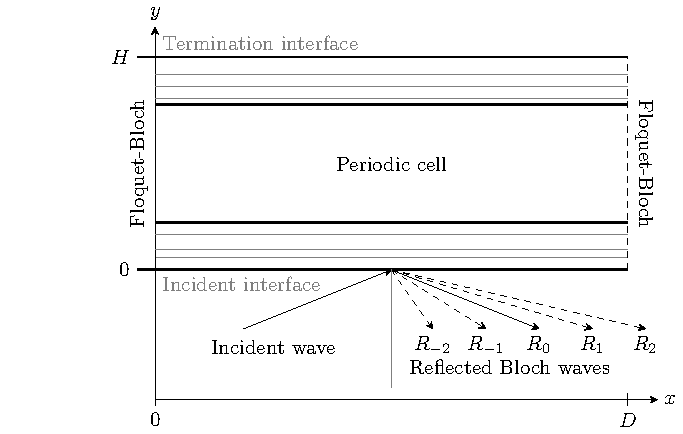
\includegraphics[width=120mm]{FIG/problem} \hfill
\caption{\label{problem} Problem of interest}
\end{center}
\end{figure}


We are interested in the problem presented in \cref{problem} corresponding to the acoustic response of a flat multilayered structure composed of homogeneous layers and periodic cells. Let $D$ be the period of the cell. The structure (of total height $H$) is assumed to be infinite in the perpendicular direction and subjected to an incident plane wave at pulsation $\omega$ with an angle $\theta$ to the normal of the panel. On top of the structure, a termination condition is imposed. It can be a rigid boundary or radiation in an infinite air medium. In all this paper, a positive Fourier transform convention is used and the common $e^{j\omega t}$ (with $j^2=-1$) term is omitted in all expressions. The incident pressure is expressed as: 
\begin{equation}
  p_i(x,y) = e^{-j(k_x x+k_y y)}
\end{equation}
The amplitude of the incident field is unity, as the physical system is linear. The wave numbers in the $x$ and $y$ directions are defined by 
\begin{equation}
 k_x=\dfrac{\omega}{c_0}\sin(\theta) \esp k_y=\dfrac{\omega}{c_0}\cos(\theta), 
\end{equation}
with $c_0$ the celerity of acoustic waves in the air. The reflected field $p_r$ is, due to periodicity of the structure, composed of a countable superposition of Bloch modes:
\begin{equation}\label{eq:p_r as R}
  p_r(x,y) = \suminf  R_w e^{-j[k_x^{(w)} x-k_y^{(w)} y]}
\end{equation}
with
\begin{equation}
  k_x^{(w)}=  k_x+ \dfrac{w\pi}{D} \esp k_y^{(w)}= \sqrt{k_0^2-{k_x^{(w)}}^2}.
\end{equation}
$R_w$ corresponds to the reflection coefficient of wave $w$. Note that the origin of the reflected waves is chosen at the incident interface. The separation of the $x$ and $y$ dependences always plays a role in these approaches. Let $\ew$ be the function of $x$ that represents the dependence on $x$. One has the following:
\begin{equation}\label{eq:definition_ew}
  \ew(x)=e^{-jk_x^{(w)} x} \esp  p_r(x,y) = \suminf  R_w \, e^{jk_y^{(w)}y} \ew (x)
\end{equation}
One key property of these functions is their orthogonality: 
\be
  \forall\, w, w'\in \Z \esp <\ew,e_{w'}> = \int_0^D \ov{\ew(x)}e_{w'}(x)dx 
  =  D\delta_{ww'} .
\ee 
The overline bar represents the complex conjugation.\\

On the top interface, a termination condition is imposed. It can be a rigid boundary or a radiation condition in an infinite medium. The rigid termination condition corresponds to zero displacement. For a transmission condition, the transmitted pressure is defined as 
\begin{equation}\label{eq:p_t as T}
  p_t(x,y) = \suminf  T_w \,e^{-jk_y^{(w)} (y-H)}\,\ew(x), 
\end{equation}
where $T_w$ are the transmission coefficients. Their origin is chosen at the termination interface. \\

The number of Bloch modes is infinite. In practice, a truncation is always performed. An integer $N$ will be defined and all sums will be truncated to $-N\leqslant w \leqslant N$.  The total number of Bloch modes is then 
\be
n_B=2N+1.
\ee 
A discussion on the choice of $N$ is presented in \cref{sec:truncation}.

\section{Models for the propagation in multilayers}

In this section, we present the different methods.  They are the GM whose unknowns are the amplitudes of the waves propagating in the different layers and the TMM. These methods were initially developed for multilayers that comprise only homogeneous layers. We will therefore modify them slightly to take into account the presence of Bloch modes in homogeneous layers. \cref{sec:homogeneous_layers} presents the modifications in the case of homogeneous layers. For periodic layers, in \cref{sec:periodic_layers} we propose an original method to relate physical quantities at the interfaces. The interface relations are presented in \cref{sec:interface_relations} and the methods for obtaining the multilayer response are then presented in \cref{sec:multilayer_response}
.\\


One of the main characters of this work is the state vector $\vc{S}$, which gathers a list of relevant physical fields that represent the dynamics of the layer. In the context of a homogeneous layer and in the absence of Bloch modes, the number of components of this vector is $2n_w$ where $n_w$ is the number of waves in the layer.  The second and third columns of \cref{tab:Physical variables} show the value of $n_w$ and a selection of fields in $\vc{S}$ for elastic, fluid, and poroelastic materials. Chapter 11 of \cite{allardPropagationSoundPorous2009a} contains more details on state vectors.\\

\begin{table}[hbtp]
  \begin{center}
    % \[\def\arraystretch{2.6}
  \begin{tabular}{||c|c|c|c|c|c||} 
  \hline \hline
  {Medium}  & {$n_w$}&{State variables $\vc{S}$} &{Primal variable $\pv$} &{Dual variable $\dv$} 
  \\ \hline
  {Fluid}& {1}&{$\left\{ u_y, p \right\}$}  & {$p$} & {$\dfrac{1}{\rho\omega^2} \dfrac{\p p}{\p n} 
  $} 
  \\ \hline
  {Elastic}& {2}& {$\left\{ \sigma_{xy}, u_y, \sigma_{yy}, u_x\right\}$}  & {$\vc{u}^e$} & {$\bs{\sigma}^e\pt\vc{n} $}  
  \\ \hline
  {Poroelastic} & {3}& {$\left\{ \hat{\sigma}_{xy}, u_y^s, u_y^t,\hat{\sigma}_{yy}, p, u_x^s\right\}$} & {\uP} & {$\left\{\bs{\hat{\sigma}}^s\pt\vc{n},\, \dfrac{1}{\rho\omega^2} \dfrac{\p p}{\p n} \right\}$} 
  \\ \hline
  % {Poroelastic 01} & {3}& {$\left\{ {\sigma}^t_{xy}, u_y^s, w_y,{\sigma}^t_{yy}, p, u_x^s\right\}$} & {\uP} & {$\left\{\bs{\sigma}^t\pt\vc{n},\, \vc{w}\pt\vc{n} \right\}$} 
  % \\ \hline
  \end{tabular}
  \caption{\label{tab:Physical variables}Variables for plane waves and finite-element methods}
  \end{center}
\end{table}



The interface relations will relate the state vectors at the interfaces between two layers. In order to avoid confusion with $\vc{S}$, which is a function of space, a specific notation is considered for the values of state variables at the interface: $\vc{\Sigma}$. Throughout this section, we will use the superscripts $t$ and $b$ to designate the quantities at the top and bottom interfaces of each layer (e.g. $y^t$ and $y^b$ will designate the coordinates of the upper and lower interfaces). We will also define a number of quantities whose expressions on the top and bottom interfaces only differ by superscript. In order not to overload the reader, we have decided to present only the expressions associated with the top interface.\\


\subsection{Homogeneous layers\label{sec:homogeneous_layers}}


The response of homogeneous layers in multilayer structures comprising periodic cells differs relatively little from the case of homogeneous multilayers. The only difference is that we have to take the Bloch modes into account. So for a given angle of incidence, we don't have just one state vector but an infinite number: one per Bloch mode. However, because of their decoupling, the relationships between the state vectors can be written separately for each wave. So, in addition to extending the method to the problem under consideration, the aim of this section is mainly to define the quantities and definitions that will be used throughout the work.\\


Inside the layer, the state vector $\vc{S}$ is defined as a function of the $x$ and $y$ coordinates and is the superposition of the contributions of the different Bloch modes:
\be 
\vc{S}(x,y) = \sumN \ew(x)\vc{S}_{w}(y)
\ee 
$\vc{S}_{w}$ is associated to a Bloch mode $w$ and can be written as a superposition of forward and backward waves travelling in the $y$ direction:
\be\label{eq:S_w forward-backward}
\vc{S}_w(y) =\sum_{\tau \in\mc{T}}  \vc{S}_{w,\tau }^+e^{-jk_\tau ^{(w)} (y-y_b)}\,q_{\w,\tau }^+ +\vc{S}_{w,\tau }^- e^{jk_\tau ^{(w)} (y-y_t)}\, q_{w,\tau}^-.
\ee 
$\mc{T}$ is the set of plane waves (compressional, shear ...) travelling in the considered layer. $\vc{S}_{w,\tau}^\pm$ is the vector of polarisations associated with the forward wave of type $\tau$ and the Bloch mode $w$. $k_\tau ^{(w)}$ is its associated projection $y$ of the wave vector and $q_{w,\tau}^\pm$ corresponds to the amplitudes. Similar definitions are introduced for backward waves but with the exponent $+$ replaced by $-$. Note that the origin of the forward waves (resp. backward) is chosen at $y=y_b$ (resp. $y=y_t$) so that this expression only involves decaying exponential terms in the $y$ direction.\\

It is more convenient to write \cref{eq:S_w forward-backward} in matrix form as:
\be
\vc{S}_w(y) =\mat{S_{\textit w}}\mat{E_{\textit w}(\textit y)}\vc{q_w} .
\ee 
$\mat{S_{\textit w}}$ is a matrix that gathers the polarisation vectors, $\mat{E_{\textit w}(\textit y)}$ is a diagonal matrix associated with the exponential terms, and $\vc{q_w}$ is the vector of the amplitudes of waves associated with Bloch mode $w$. At the top interface, one has:
\be\label{eq:state_top}
\vc{\Sigma}^t_{w}=\vc{S}_w(y^t)= \mat{S_{\textit w}}\mat{E_{\textit w}(\textit y^t)}\vc{q_w}
\ee 

The transfer matrix $\mat{T_{\textit w}}$ associated with the Bloch mode $w$ relates the state vector at the top interface to the state vector at the bottom interface:
\begin{equation}\label{eq:transfer_matrix}
  \vc{\Sigma}^b_{w} = \mat{T_{\textit w}}\vc{\Sigma}^t_{w}
\end{equation}
Its expression is as follows.
\begin{equation}
  \mat{T_{\textit w}} = \mat{S_{\textit w}}\mat{E_{\textit w}(\textit y_{\textit b})}
  \mat{E_{\textit w}(\textit y_{\textit t})}^{-1}
  \mat{S_{\textit w}}^{-1}
\end{equation}
Global state vectors can be defined gathering the state vectors associated to selected Bloch modes: 
\be\label{eq:state_top_allmodes}
\vc{\Sigma}^t = \Big\{
    \vc{\Sigma}^b_{-N},\, \hdots ,\, \vc{\Sigma}^b_{0} ,\, \hdots ,\,\vc{\Sigma}^b_{N} \Big\} \in \C^{n_\Sigma}\esp n_\Sigma = 2n_wn_B.
\ee 
They can be also expressed as a function of the amplitudes of the global waves amplitudes $\vc{q}$ in a form similar to \cref{eq:state_top}:
\be\label{eq:state_top_allmodes_q}
\vc{\Sigma}^t = \mat{\Xi^t}\vc{q} \esp \vc{q}=\Big\{
    \vc{q}_{-N},\, \hdots ,\, \vc{q}_{0} ,\, \hdots ,\,\vc{q}_{N} \Big\}  
\ee
Note that $\mat{\Xi^t}$ is diagonal by block, each block being $\mat{S_{\textit w}}\mat{E_{\textit w}(\textit y^t)}$ so that this matrix gathers both polarisations and exponential terms. $\vc{\Sigma}^b$ and $\vc{\Sigma}^t$ are related by a global transfer matrix $\mat{T}$ that is diagonally orientated by blocks, each block $\mat{T_{\textit w}}$ (for $w=-N,\hdots ,\, N$) being defined as in \cref{eq:transfer_matrix}: 
\be\label{eq:transfert_allmodes}
\vc{\Sigma}^b_w= \mat{T_w}\vc{\Sigma}^t_w \so \vc{\Sigma}^b = \mat{T}\vc{\Sigma}^t.
\ee 
Note that formally, one has:
\be 
\mat{T}=\mat{\Xi^b}\mat{\Xi^t}^{-1}.
\ee 



\subsection{Case of periodic cells\label{sec:periodic_layers}}

% \begin{figure}[hbtp]
% \begin{center}
% 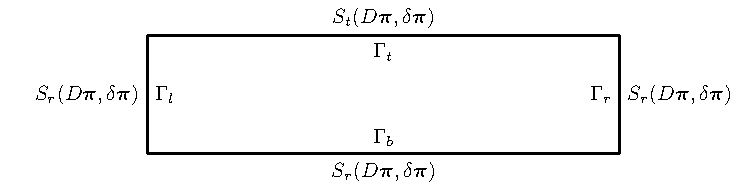
\includegraphics[width=120mm]{FIG/periodic_cell} \hfill
% \caption{\label{periodic_cell} Periodic cell}
% \end{center}
% \end{figure}

The case of periodic cells is now presented. We will couple FEM to state vectors $\vc{\Sigma}^t$ and $\vc{\Sigma}^b$ on the top and bottom interfaces. The cell is associated with a volume $\Omega$ bounded by a rectangle of the boundary $\Gamma$. $\Omega$ can be filled by an aggregate of different media but we will consider that each cell is composed of a core material which covers the upper and lower boundaries. This weak form involves two terms: a volume term associated with the primal variable $\pv$ and a boundary term associated with the dual variable $\dv$.\\


The key idea of the proposed method is that state variables allows to corresponds to the aggregate of primal and dual variables, as illustrated in \cref{tab:Physical variables}. First, the state vector $\vc{S}^t$ is a function of $x$ whose relation with $\vc{\Sigma}^t$ is: 
\be\label{eq:state_top_periodic}
\vc{S}^t(x) = \sumN \ew(x)\vc{\Sigma}^t_{w} \so
\vc{S}^t(x) = \mat{\Lambda(\textit x)}\vc{\Sigma}^t
\ee
$\mat{\Lambda(\textit x)}$ is a matrix $2n_w \times 2n_wn_B$ that gathers the exponential terms $\ew(x)$. It reads:
\be
\mat{\Lambda(\textit x)} = \begin{bmatrix}
  e_{-N}(x)\mat{I} & \hdots & e_{N}(x)\mat{I}
\end{bmatrix} =  \vc{e(\textit x)}\otimes\mat{I}\, \tr{with} \,\vc{e(\textit x)}=[
  e_{-N}(x),\, \hdots ,\, e_{N}(x)
]
\ee  
where $\mat{I}$ is the identity matrix of dimension $2n_w$.\\

Second, two boolean matrices $\mat{\pv}$ and $\mat{\dv}$ of dimension $n_w \times 2n_w$ can be defined to relate the FEM variables to the state variables.
\begin{subequations}
\be
\label{eq:identification pv to S}
\pv(x,y=y_t) = \mat{\pv}   \mat{\Lambda(\textit x)}\vc{\Sigma}^t \esp 
\ee
\be\label{eq:identification dv to S}
\dv(x,y=y_t) = \mat{\dv}    \mat{\Lambda(\textit x)}\vc{\Sigma}^t
\ee 
\end{subequations}
Note that $\vc{\pi}$ and $\vc{b}$ are considered vectors insofar as the primal variables can be associated with several physical fields.\\

The weak form associated with $\Omega$ can be written in the form:
\begin{equation}\label{eq:weak_form}
\forall \test \in V \esp  a(\pv,\test)=\int_{\Gamma} 
 \test(M)\tp \dv(M)  dS
\end{equation}
$a$ is a bilinear form that is defined in the space $V$ of admissible functions. $\test\in V$ is a test function, and $\tp$ is the real transposition. $\Gamma$ can be decomposed into four edges $\Gamma_t$, $\Gamma_b$, $\Gamma_l$ and $\Gamma_r$, respectively, associated with the top, bottom, left and right edges of the cell so that \cref{eq:weak_form} can be written as:
\begin{equation}\label{eq:weak_form_decomposed}
  a(\pv,\test)-\int_{\Gamma_l\cup \Gamma_r} 
\test(y)\tp \dv(y)  dy
=\int_{\Gamma_t} 
\test(x)\tp \mat{\dv}    \mat{\Lambda(\textit x)}\vc{\Sigma}^t  dx 
 +\int_{\Gamma_b} 
\test(x)\tp \mat{\dv}    \mat{\Lambda(\textit x)}\vc{\Sigma}^b  dx 
\end{equation}
Imposition of \cref{eq:identification pv to S} is done in a weak sense by projection on the $\ew$ functions:
\be\label{eq:weak_form_pv}
\int_{\Gamma_t} \ov{\ew(x)} \pv(x)dx=
 \int_{\Gamma_t} \ov{\ew(x)} \mat{\pv}   \mat{\Lambda(\textit x)}\vc{\Sigma}^tdx
\ee 
Due to the orthogonality of the functions $\ew$, one as:
\be
 \int_{\Gamma_t} \ov{\ew(x)} \mat{\pv}   \mat{\Lambda(\textit x)}\vc{\Sigma}^tdx=
 D \mat{\pv} \vc{\Sigma}^t_w.
\ee 

This relationship therefore corresponds to the calculation of the contributions of the Bloch modes using the primal variables of the finite element model. Hence, for each primal variable $\pi_k\in\vc{\pi}$ and each Bloch mode $w$:
\be\label{eq:rothogonality_pv}
 \int_{\Gamma_t} \ov{\ew(x)} \pi_k(x)dx=
  D \Sigma^t_{k,w},
\ee
where $\Sigma^t_{k,w}$ is the component of the state vector associated with the Bloch mode $w$ and field $\pi_k$.\\
\\ 


Let us come to the discretization of the system made up of equations (\ref{eq:weak_form_decomposed}) and (\ref{eq:rothogonality_pv}).
The first one is discretised with higher order finite-elements. The primal variable is approximated as: 
\be
\pv(M) = \mat{N(\textit M)}\vc{X}\esp \delta\pv(M) = \mat{N(\textit M)}\delta\vc{X}
\ee 
where $\mat{N(M)}\in \mb{R}^{n_w\times n}$ is the matrix of shape function and $\vc{X}\in\mb{R}^n$ is the vector of the finite-element unknowns. The restriction of the variable $\pi_k$ on the upper interface leads to: 
\be
\pi_{k|y=y_t}(M) = \mat{N_t^k(\textit M)}\vc{X}\esp 
\mat{N_t^k(\textit M)} \in\mb{R}^{1\times n}.
\ee
The full vector of the primal variables can then be discretised as:
\be
\pv_{|y=y_t}(M) = \mat{N_t(\textit M)}\vc{X}\esp 
\delta \pv_{|y=y_t}(M) = \mat{N_t(\textit M)}\delta\vc{X}
\ee 




This method has now been widely used in the literature; see, for instance, \cite{petytIntroductionFiniteElement2010,atallaFiniteElementBoundary,solinHigherorderFiniteElement2004}, and is then not detailed in the present work. The term $a$ associated with the volumic term leads to a matrix $\mat{D_{\pi\pi}}\in \C^{n\times n}$. The term of (\ref{eq:weak_form_decomposed}) associated to $\Gamma_t$ is discretised as:
\be
\int_{\Gamma_t} 
\test(x)\tp \mat{\dv}    \mat{\Lambda(\textit x)}\vc{\Sigma}^t  dx  \approx
\delta\vc{X} 
\underbrace{\int_{\Gamma_t} 
\mat{N_t(\textit x)}\tp\mat{\dv} 
 \mat{\Lambda(\textit x)}  dx}_{\mat{D_{\pi t}}} \vc{\Sigma}^t
\ee

$\mat{D_{\pi t}}$ is a matrix of dimension $n\times n_\Sigma$ that is not classical in the sense of the FEM, as the integrand is associated to the product of polynomial by exponential functions. Its terms are based on those of $\mat{\phi}\in\C^{n\times 2N+1}$ with
\be
\mat{\phi}=\int_{\Gamma_t} 
\mat{N_t(\textit x)}\tp
 \mat{e(\textit x)}  dx
\ee
which contains all the integration of the products of the traces of finite element shape functions by exponential Bloch modes functions. Note that the terms of the latter matrix can be computed analytically. The discretization of (\ref{eq:rothogonality_pv}) leads to $n_wn_B$ equations linking $\vc{X}$ and $\vc{\Sigma}^t$. The right-hand side is discretised as: 
\be
 \int_{\Gamma_t} \ov{\ew(x)} \pi_k(x)dx \approx \underbrace{
 \int_{\Gamma_t} \ov{\ew(x)} \mat{N_t^k(\textit x)}dx}_{ \mat{D^{k,w}_{t\pi}}} \vc{X}
\ee
$\mat{D^{k,w}_{t\pi}}\in\C^{1 \times n }$ is a row matrix whose terms are conjugates of those associated with mode $w$ in $\mat{\phi}$. By gathering all the orthogonality relations, it is possible to write the relation between $\vc{\Sigma}^t$ and $\vc{X}$ as:
\be
  \mat{D_{tt}} \vc{\Sigma}^t+\mat{D_{t\pi}}\vc{X}=\vc{0}.
\ee
$\mat{D_{t\pi}}$ is built after the aggregation of the row matrices $\mat{D^{k,w}_{t\pi}}$ and $\mat{D_{tt}}\in\mb{R}^{n_wn_B\times n_wn_B}$ is the scalar matrix whose entries on the diagonal are all equal to $D$.\\

The last terms to be considered are terms associated with $\Gamma_l$ and $\Gamma_r$ in \cref{eq:weak_form_decomposed}. Due to the periodicity condition, they can be cancelled by a master-slave approach that consists of imposing that both degrees of freedom and boundary terms on the right edge are equal to those on the left edge multiplied by a phase factor $e^{jk_xD}$. This is not detailed here for the sake of concision. The final linear system associated with the periodic cell is then written as:
\be 
\begin{bmatrix}
  \mat{D_{tt}} & \mat{D_{t\pi}} &\mat{0} \\
  \mat{D_{\pi t}} & \mat{D_{\pi\pi}} &\mat{D_{\pi b}} \\
  \mat{0} & \mat{D_{b\pi}} &\mat{D_{bb}} 
\end{bmatrix} 
\begin{Bmatrix} 
\vc{\Sigma}^t \\ 
\vc{X}\\
\vc{\Sigma}^b
\end{Bmatrix}=\vc{0}.
\ee 

Let us now deduce relations between the state vectors at the top and bottom interfaces. The finite-element degrees of freedom can first be condensed as:

\be 
\vc{X}  = \mat{R_t}\vc{\Sigma}^t +\mat{R_b}\vc{\Sigma}^b
\ee 
with 
\be \mat{R_t} =-\mat{D_{\pi\pi}}^{-1}\mat{D_{\pi t}} \esp  
\mat{R_b} =-\mat{D_{\pi\pi}}^{-1}\mat{D_{\pi b}}
\label{eq:rb_rt}
\ee 
We then have:
\be\label{eq:relation_Sigmas_periodic}
\underbrace{\begin{bmatrix}
   \mat{D_{t\pi}}\mat{R_b}\\
  \mat{D_{bb}}+ \mat{D_{b\pi}} \mat{R_b}
\end{bmatrix}}_{\mat{M_b}}\vc{\Sigma}^b +
\underbrace{\begin{bmatrix}
  \mat{D_{tt}}+
  \mat{D_{t\pi}}\mat{R_t} \\
  \mat{D_{b\pi}}\mat{R_t} 
\end{bmatrix}}_{\mat{M_t}}\vc{\Sigma}^t=\vc{0}
\ee
The transfer matrix of the periodic layer is then:


\be 
\vc{\Sigma}^b =\mat{T}\vc{\Sigma}^t \tr{ with } 
\mat{T}=-\mat{M_b}^{-1}\mat{M_t}.
\ee

\subsection{Interfaces relations\label{sec:interface_relations}}

Let us now look at the relationship between the fields at the interfaces between layers. First, these are independent of whether the layers are homogeneous or periodic. To avoid confusion with what we have presented earlier, we will consider that the layer above will be marked with the subscript $a$ and the layer below with the subscript $b$. We therefore have two state vectors $\vc{\Sigma}_+$ and $\vc{\Sigma}_-$, which are composed, for each layer, of the aggregation of the contributions of each Bloch mode to the state vector. As these are orthogonal, the interface relationships are decoupled from each other.\\


The state vectors are, respectively, of length $2n_an_B$ and $2n_bn_B$ where $n_a$ and $n_b$ are the number of waves $n_w$ shown in \cref{tab:Physical variables}. The number of interface relations is equal to $n_a+n_b$ and can be written in the form:
\be
\mat{C_a}\vc{\Sigma}_a +\mat{C_b}\vc{\Sigma}_b = \vc{0},
\ee
where $\mat{C_a}\in\R^{n_a+n_b\times 2n_a}$ and $\mat{C_b}\in\C^{n_a+n_b\times 2n_b}$ are interface matrices. These matrices express the continuities between the stresses and displacements of the media in the two layers at the interface or the possible nullities of some fields. The expressions of these matrices are not given, but the reader can in particular consult Table IV of \cite{dazelStableMethodModel2013}.

\subsection{Methods to model the acoustics response of the multilayer structure\label{sec:multilayer_response}}

The two methods we are going to compare are now be presented. The proposed approach is a general one, but in the context of this section we will limit ourselves to present it in the case of a bilayer structure composed of an homogeneous layer (labeled 1) on top of a periodic cell (labeled 2) as presented in \cref{two_layers_problem}. \\ 

A state vector $\vc{\Sigma_-}\in\C^{2n_B}$ is defined on the lower side of the incident interface. It can be written as a sum of a vector $\vc{E}$ associated to the incident field and a contribution of the reflected waves: 
\be 
\vc{\Sigma}_- = \mat{\rho}\mc{R}+\vc{E} \esp \mc{R}=\{R_{-N},\hdots \, , R_N\}
\ee
$\mat{\rho}\in\C^{2\times n_B}$. It is diagonal by block, each column is associated to a Bloch mode and provides the displacement along $y$ and the pressure of the considered Bloch mode as a function of the reflexion coefficient $R_w$ of wave $w$. $\mc{R}\in\C^{n_B}$ is the vector of reflexion coefficients.\\


The termination condition can be either transmission in a semi-infinite media or a rigid wall. The first case is similar to the one of the incident interface. The state vector $\vc{\Sigma}_+$ is defined from the transmission coefficient vector $\mc{T}$ as follows:
\be
\vc{\Sigma}_+ = \mat{\tau}\mc{T} \esp \mc{T}=\{T_{-N},\hdots \, , T_N\}
\ee
$\mat{\tau}\in\C^{2\times n_B}$ is a diagonal by block matrix that relates the displacement along $y$ and the pressure of the considered Bloch mode as a function of the transmission coefficient $T_w$ of wave $w$. For that termination condition, the total number of relations at interfaces is:
\be
n_t = n_B(1+n_1)+n_B(n_1+n_2) + n_B(n_2+1)=(2+2n_1+2n_2)n_B.
\ee 


In the case of a rigid wall, the nullity of the displacement in $\vc{\Sigma}_1^t$ is imposed as 
\be
\mat{D}\vc{\Sigma}_1^t = \mat{0} \esp \mat{D}=\mat{\hat{D}}\otimes \mat{I_{n_B}}
\ee
$\mat{\hat{D}}\in\R^{n_1 \times 2n_1}$ is a boolean matrix whose non-zero entries are associated to the displacements in the state vector. The total number of boundary and interface relations is then:
\be
n_t = n_Bn_1+n_B(n_1+n_2) + n_B(n_2+1)=(1+2n_1+2n_2)n_B
\ee 


\begin{figure}[hbtp]
\begin{center}
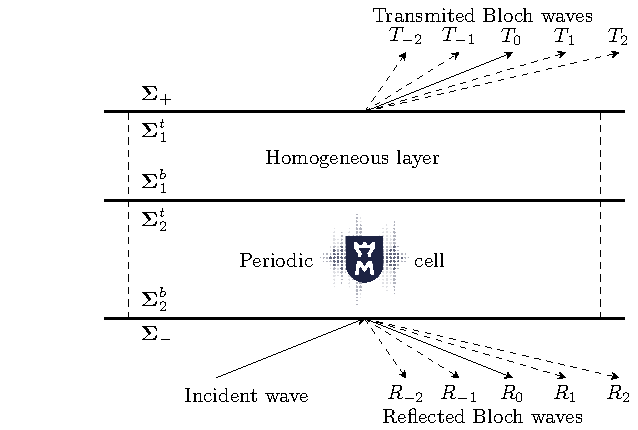
\includegraphics[width=120mm]{FIG/two_layers_problem} \hfill
\caption{\label{two_layers_problem} Two layers problem}
\end{center}
\end{figure}


\subsection{Global method}

The unknonws of the global method are the amplitudes of the waves for homogeneous layers and the top and bottom state vectors for periodic layers. In the case of a transmission condition, the system of equations is written as follows:
\be\label{eq:Global method system}
\begin{bmatrix}
\mat{C_+}\mat{\tau} & \mat{C_1^t}\mat{\Xi^t}\ & \mat{0} & \mat{0} & \mat{0}\\
\mat{0} & \mat{C_1^b}\mat{\Xi^b}\ & \mat{C_2^t} & \mat{0} & \mat{0} \\
\mat{0}&\mat{0}&\mat{M_t} & \mat{M_b} & \mat{0} \\
\mat{0}&\mat{0}&\mat{0}&\mat{C_2^b} & \mat{C_-} \mat{\rho}
\end{bmatrix}
\begin{Bmatrix}
  \mc{T}\\
  \vc{q}_1\\
  \vc{\Sigma}_2^t\\
  \vc{\Sigma}_2^b\\
  \mc{R}
\end{Bmatrix}=\begin{Bmatrix}
  \vc{0}\\
  \vc{0}\\
  \vc{0}\\
  -\mat{C_b^1}\vc{Inc}
\end{Bmatrix}
\ee 
The number of unknowns is $n_B$ for both $\mc{T}$ and $\mc{R}$, $2n_1n_B$ for $\vc{q}_1$ and $2n_2n_B$ for $\vc{\Sigma}_2^t$ and $\vc{\Sigma}_2^b$. The first and second block rows correspond to $n_B(1+n_1)$ (resp. $n_B[n_1+n_2])$ continuity relations at the transmition (resp. second interface). The third block row corresponds to the $2n_Bn_2$ relations of \cref{eq:relation_Sigmas_periodic} and the last block row to the $n_B(n_2+1)$ relation at the incident interface. In the case of a rigid termination, $\vc{T}$ is no longer in the unknowns, and the first block column disapears. In addition, $\mat{C_b^1}\mat{\Xi^t}$ is replaced by $\mat{D}\mat{\Xi^t}$ corresponding to $n_1n_B$ relations. Hence, in both cases, the relations are independent, and their number is equal to the number of unknowns. As the origin of waves is at the adequate interface, this system only involves decaying exponentials.\\ 


\subsection{Transfer Matrix Method}

The unkowns of the TMM are the state vectors on the top interfaces of each layer, $\mc{R}$ (and $\mc{T}$  in the case of a transmission medium). The expression of state vectors on the bottom interfaces are obtained by a multiplcation by the transfer matrices of each layer. The system of equations is then written as follows:
\be
\begin{bmatrix}
\mat{C_+}\mat{\tau} & \mat{C_1^t} & \mat{0} & \mat{0}\\
\mat{0} & \mat{C_1^b}\mat{T_1}\ & \mat{C_2^t}  & \mat{0} \\
\mat{0}&\mat{0}&\mat{C_2^b}\mat{T_2} & \mat{C_-} \mat{\rho}
\end{bmatrix}
\begin{Bmatrix}
  \mc{T}\\
  \vc{\Sigma}_1^t\\
  \vc{\Sigma}_2^t\\
  \mc{R}
\end{Bmatrix}=\begin{Bmatrix}
  \vc{0}\\
  \vc{0}\\
  -\mat{C_b^1}\vc{Inc}
\end{Bmatrix}
\ee 
When the multilayer comprises a succession of several materials of the same type, the lower interface corresponds to that of the last layer and the transfer matrix corresponds to the product of the matrices of the successive layers. The succession is thus treated as a single layer. 


\section{Results}

\subsection{Validation on homogeneous multilayer structures}

The main goal of these first two examples is to compare the different methods applied to a homogeneous multilayered structures case and to show that the errors for each method are identical. The first problem is that of a 1 meter square air cavity, excited by a plane wave at normal incidence ($k_x=0)$. The cavity, described as a periodic cell with periodicity $D=1$ m and thickness $H=1$ m, is modeled using FEM and discretized by 2 triangular elements. A rigid boundary condition is applied on top. For this simple case, it is easy to obtain the reflection coefficient for this problem, which serves as the reference solution: 
\begin{equation}
    R= \dfrac{Z_s-1}{Z_s+1} \esp 
    Z_s =-j\cot\left(kH\right) \esp k=\dfrac{\omega}{c_0}.
\end{equation}

Three methods are compared in this example and are all associated to the same mesh: the GM and TMM methods presented in \cref{sec:multilayer_response} as well as a FEM resolution in which a unit velocity is imposed at the bottom boundary, the three other ones are associated to rigid walls. The surface impedance $Z_s$ can then be deduced from the pressure on this boundary and finally the reflection coefficient. This method serves as an indicator on the convergence of the FEM. The diagram of the configuration is depicted in Fig.~\ref{Air cavity_mesh} and the error for each method is given in Fig.~\ref{Air cavity_error}. There, the convergence for each method is shown depending on the adimensional parameter $kH$ and for different interpolation orders $p=2$ to 7. At each order, the errors of each of the four methods are perfectly superimposed (except when the error reaches the machine precision). All methods lead to the same error as the direct FEM resolution, thus indicating that there is no other additional source of error than the FEM approximation.

\begin{figure}[hbtp]
\centering
\begin{subfigure}{.5\textwidth}
  \centering
  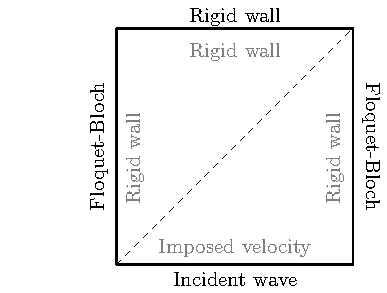
\includegraphics[width=\linewidth]{FIG/cavity}
  \caption{Geometry of the problem. Boundary conditions in black (resp.gray) are for the proposed methods (resp. the FEM reference).\label{Air cavity_mesh}}
  
\end{subfigure}%
\begin{subfigure}{.5\textwidth}
  \centering
  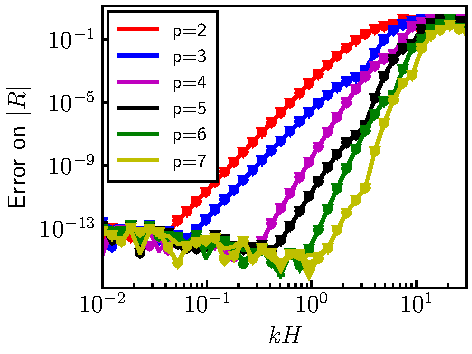
\includegraphics[width=\linewidth]{FIG/Convergence_Air_layer}
  \caption{solid line: FEM reference: +: Global Method, $\triangledown$: TMM\label{Air cavity_error}}
\end{subfigure}
\caption{Convergence of the reflection coefficient for an air cavity excited by a plane wave under normal incidence for several interpolation orders}
\label{fig:test}
\end{figure}



\begingroup
\renewcommand*{\arraystretch}{1}
\begin{table}[hbtp]
	\begin{center}
	\begin{tabular}{lcccc} 
	\hline
 \textbf{Parameter}&\textbf{PEM 1} & \textbf{PEM 2} & \textbf{Rubber} & \textbf{Steel}\\ 
 \hline
    Porosity $\phi \,[\emptyset]$   					& 0.989 & 0.95& / &/\\
    Resistivity $\sigma\,[ N.s.m^{-4}]$ 				& 8060 & 42 000&/ &/\\
    Tortuosity   $\alpha_\infty\,[\emptyset]$ & 1.0 & 1.1& /& /\\
    Viscous characteristic length  $\Lambda\,[\mu m]$ 			& 214 & 15& / &/\\
    Thermal characteristic length  $\Lambda'\,[\mu m]$ 			& 214  & 45& /&/\\
    Density	 $\rho\,[kg.m^{-3}]$ & 6.1 & 126 & 1800&7800\\
    Young's modulus $E \,[kPa]$ & 56.5 & 694.4& 1900&49.7$\times 10^6$\\
    Poisson's ratio $\nu \,[\emptyset]$ 					& 0.24&0.24&0.48&0.45 \\
    Frame loss model  &structural &structural &rubber&none\\
    Structural loss factor $\eta \,[\emptyset]$ 					& 0.02 & 0.05 &796&0\\
	\hline
	\end{tabular}
	\end{center}
	\caption{Physical parameters of the different media}
	\label{tab:param_mat}
\end{table}
\endgroup

A second validation case is presented in Fig.~\ref{Convergence_sandwich_mesh} with the transmission problem of sandwich structure of two rubber coatings ($h=0.2$ mm) surrounding a poroelastic layer of PEM 1 ($h=2$ cm) immerged in two semi-infinite air media. Note that in \cref{Convergence_sandwich_mesh}, the rubber coatings are hardly visible due to their very thin thickness. The excitation angle is $60^o$. In this example, we have chosen to model the air layers (with a thickness of 20 cm) for several reasons: to ensure that the method is properly implemented (especially the elastic-fluid coupling), to check that the phase shift induced by the propagation in the two air layers are properly captured, and because in several choices of FEM implementation, they need to be modelled (and are generally coupled to PML). We point out that the objective of this subsection is to test the method rather than to obtain the most efficient model. The reference reference solution is computed through the RM. \\

This structure can then be considered as a five-layer stack, and three different approaches are considered to test the implementation. The first one (called entire structure) is to consider that this is a stack of five periodic cells. The second approach (called sandwich structure) accounts for the modelling of the two air layers as homogeneous materials and the 3 layer stack as a periodic cell. Note that in that case the FEM model of the periodic cell is composed of two different materials (PEM 1 and rubber). In the last case (called the poroelastic core), only the porous material is modelled as a periodic cell, and the rubber and air layers are considered as homogeneous materials. The period $D$ is 1 meter and the periodic cell meshes are created independently of each other, with a characteristic size $h$. Note that the different meshes may not be compatible at the interfaces, which is not a problem for the proposed methods.\\

The error on the modulus of the transmission coefficient is presented in \cref{Convergence_sandwich_error}. In order not to overload the figure, only the results with the GM are presented but the TMM matches at machine precision. For each order the errors of the three models are perfectly superposed (except for coarse meshes where the FE models are not converges and for fine meshes and order higher than 6 where the systems at ill-conditioned). This is validate the approach but also indicate that, in that problem, the error is governed by the one of the poroelastic core. We can also draw the conclusion that it is obviously superfluous to discretize homogeneous layers by finite elements. In the following cases, only periodic layers will be modelled using finite elements and the homogeneous layers will be modelled using plane waves.

\begin{figure}[hbtp]
\centering
\begin{subfigure}{.5\textwidth}
  \centering
  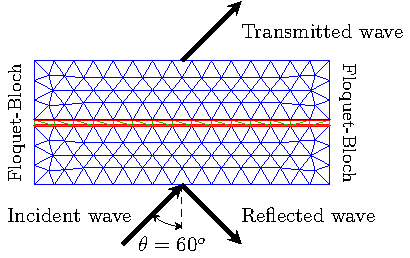
\includegraphics[width=0.9\linewidth]{FIG/meshes_sandwich.pdf}
  \caption{Coupled vibroacoustic sandwich problem}
  \label{Convergence_sandwich_mesh}
\end{subfigure}%
\begin{subfigure}{.5\textwidth}
  \centering
  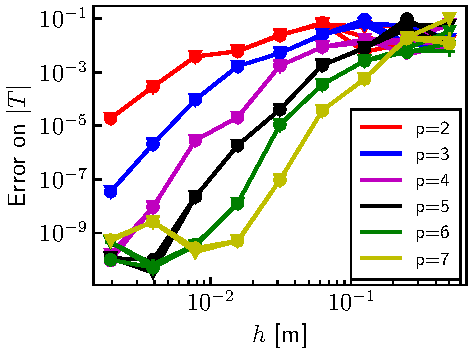
\includegraphics[width=\linewidth]{FIG/Convergence_sandwich_lcar_error.pdf}
  \caption{\label{Convergence_sandwich_error} (+) poroelastic core, ($\triangledown$) sandwich structure, (o) entire structure }
\end{subfigure}
\caption{Convergence curve for the global method for the problem of a sandwich structure}
\label{fig:sandwich}
\end{figure}


\subsection{Validation on metaporous structures}

In this subsection, we will compare the two methods with examples inspired by the literature on metaporous structures. The first is a poroelastic core ($D=H=2$ cm) with an embedded steel inclusions (of radius 8 mm) with a rigid backing studied in \cite{weisserAcousticBehaviorRigidly2016a} and depicted in \cref{fig:schema_benchmark}a. The second is a two side rubber-coated poroelastic slab with a resonant air-filled rubber shell inclusion (case b presented in figure 2 of \cite{gaboritCouplingFEMBloch2018}) (\cref{fig:schema_benchmark}c).\\

\begin{figure}[hbtp]
    \centering
    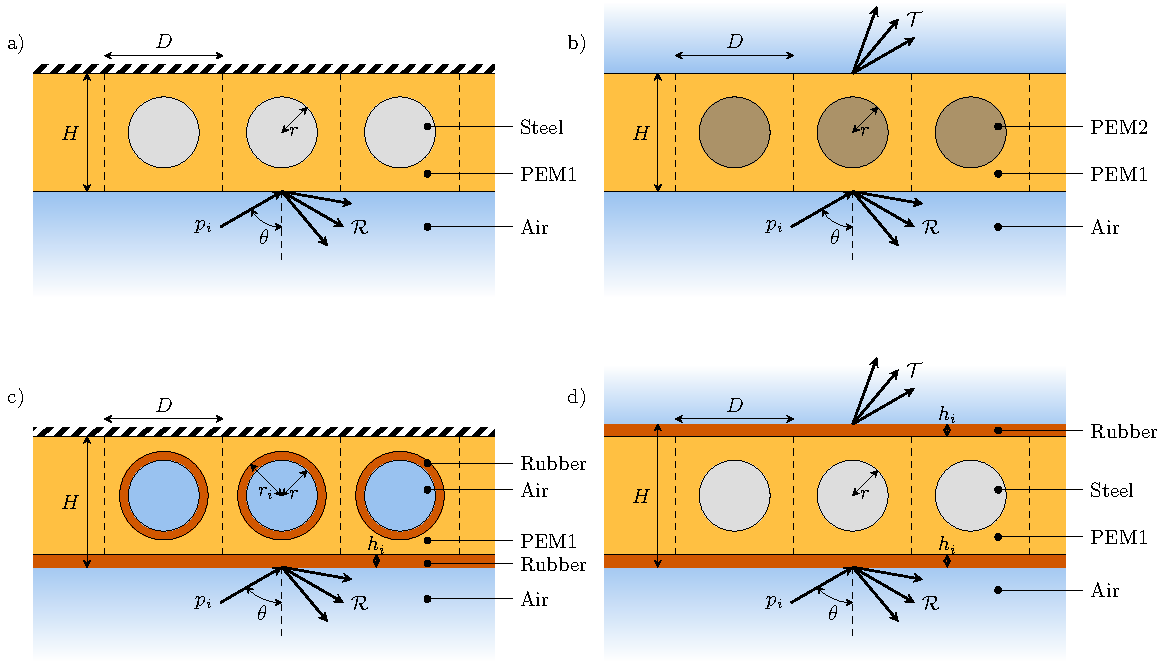
\includegraphics[width=\linewidth]{FIG/schema_benchmark.pdf}
    \caption{Diagram for the presented cases, each case is a poroelastic host layer, a) rigidly-backed and steel inclusions, b) transmission problem with embedded poroelastic inclusions, c) rigidly-backed with a rubber-coating and resonant air-filled rubber shell, d) transmission problem with a rubber-coating on each side and steel inclusion}
    \label{fig:schema_benchmark}
\end{figure}

\cref{fig:case1} presents the results for the first case. The number of Bloch waves is chosen as $N=2$ and the size of the mesh is $h=D/5=4~\mathrm{mm}$. The results are presented for two incident angles ($\theta=0^o$ and $\theta=30^o$). The absorption curves presented in \cref{fig:case1_abs} are superimposed to the multiple scattering solutions which is considered as the reference. In this figure, only the results obtained by the Global Method are presented but the TMM results are very close. More precisely, their error to the reference solution are presented in \cref{fig:case1_error}. They coincide for both angles, except at low frequencies where errors are around $10^{-5}$. It is worth noticing that the maximum error is around 4000 Hz (around $10^{-3}$ and is due to Biot effects. It can be reduced by refining the mesh.

\begin{figure}[hbtp]
\centering
\begin{subfigure}{.5\textwidth}
  \centering
  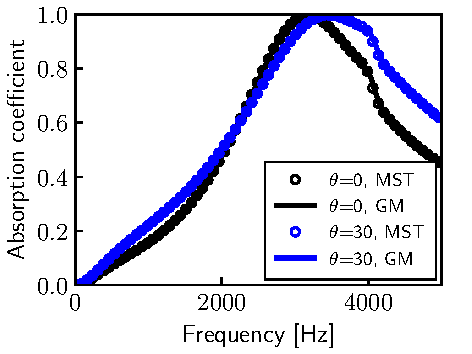
\includegraphics[width=\linewidth]{FIG/case1_abs}
  \caption{Absorption coefficient at two angles\label{fig:case1_abs}}
\end{subfigure}%
\begin{subfigure}{.5\textwidth}
  \centering
  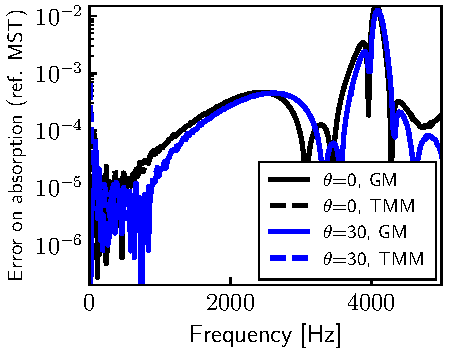
\includegraphics[width=\linewidth]{FIG/case1_error}
  \caption{Errors of the methods.\label{fig:case1_error}}
\end{subfigure}
\caption{Case of a elastic inclusion in a porous material \cite{weisserAcousticBehaviorRigidly2016a}. Solid (resp. dashed) lines correspond to $\theta=0^o$ (resp. $\theta=30^o$)  \label{fig:case1}}
\end{figure}

Similar conclusions can be observed in the second case presented in \cref{fig:case13}. The number of Bloch waves is $N=3$ and the characteristic size of the mesh is $h=D/40=0.5\, \mathrm{mm}$ so as to capture the resonance of the inclusion. The level of error presented in \cref{fig:case13_error} is very low indicating the good prediction obtained by the three methods. Nevertheless, a closer look at the errors above 3000 Hz shows small oscillations in the TMM, suggesting stability issues that we will investigate now more in detail.

\begin{figure}[hbtp]
\centering
\begin{subfigure}{.5\textwidth}
  \centering
  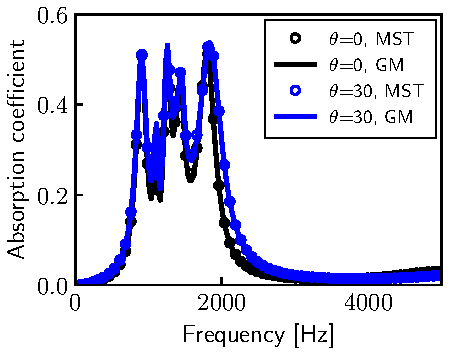
\includegraphics[width=\linewidth]{FIG/case13_abs}
  \caption{Absorption coefficient at two angles\label{fig:case13_abs}}
\end{subfigure}%
\begin{subfigure}{.5\textwidth}
  \centering
  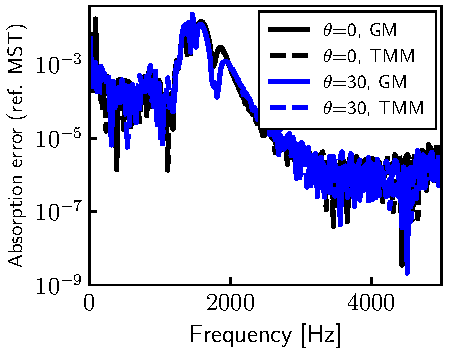
\includegraphics[width=\linewidth]{FIG/case13_error}
  \caption{Errors of the three methods\label{fig:case13_error}}
\end{subfigure}
\caption{Case of a two-sided coated  of a resonant inclusion in two side coated  material. Solid (resp. dashed) lines correspond to $\theta=0^o$ (resp. $\theta=30^o$)  \label{fig:case13}}
\end{figure}

\subsection{Stability issues }
This part is dedicated to highlighting the stability issues that arise with the TMM. The configuration presented in \cref{fig:schema_benchmark}d is used. \cref{fig:case13_abs} is showing matching results to the reference for the absorption curves computed using GM and two Bloch truncation values $N=3$ and $N=7$. The error profile also shows that the error is the same for both truncations at low frequencies. However, in the mid-frequency range, greater precision is achieved by accounting more Bloch modes since higher frequencies generally require the progressive addition of Bloch modes to the series. This behaviour shows a satisfying stability for the GM, seemingly able to account for a large amount of Bloch waves without loss of precision. 

However, the TMM results compared to the same reference is showing large discrepancies on its absorption profile at lower frequencies in the case $N=3$. These results are made worse with a growing amount of Bloch waves taken into account $N=7$, where the absorption response does not match the reference over the whole frequency range, as shown also with the condition number gaining around 10 orders of magnitude for the TMM when going from 3 to 7 Bloch waves in the truncation. This also shows that the conditioning of the GM global matrices remains tame with an increasing amount of Bloch waves, as observed in the previous paragraph. The inherent instability of the TMM shows some limitations in this particular configuration as highlighted by this result. This has also been observed for a wide range of numerical experiments that we have performed and not shown in the present work. Moreover, unstability of the TMM is a common feature \cite{loweMatrixTechniquesModeling1995}. We point out that in our implementation of the GM for periodic cell, the stablility is preserved as both $\vc{\Sigma}^t$ and $\vc{\Sigma}^b$ are unknowns of \cref{eq:Global method system} and not just one of them.

\begin{figure}[hbtp]
\centering
\begin{subfigure}{.5\textwidth}
  \centering
  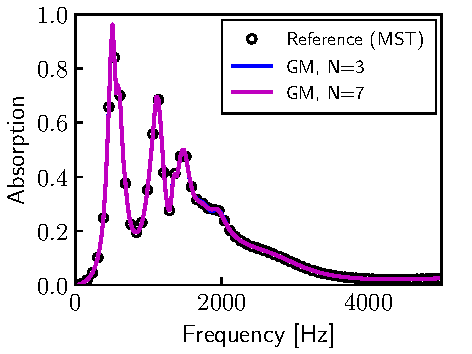
\includegraphics[width=\linewidth]{FIG/case10_abs_global}
  \caption{Absorption coefficient\label{fig:case10_abs_global}}
\end{subfigure}%
\begin{subfigure}{.5\textwidth}
  \centering
  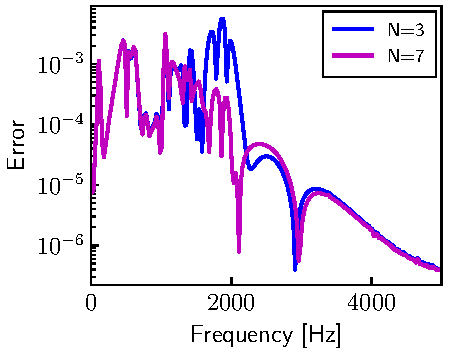
\includegraphics[width=\linewidth]{FIG/case10_error_global}
  \caption{Error on the absorption \label{fig:case10_error}}
\end{subfigure}
\caption{Prediction of the GM for two truncation of the Bloch modes \label{fig:case10_global}}
\end{figure}


\begin{figure}[hbtp]
\centering
\begin{subfigure}{.5\textwidth}
  \centering
  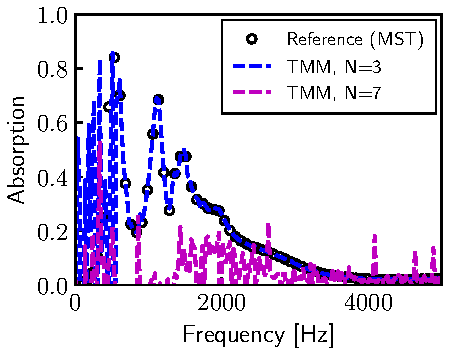
\includegraphics[width=\linewidth]{FIG/case10_abs_TMM}
  \caption{Absorption coefficient\label{fig:case10_abs_others}}
\end{subfigure}%
\begin{subfigure}{.5\textwidth}
  \centering
  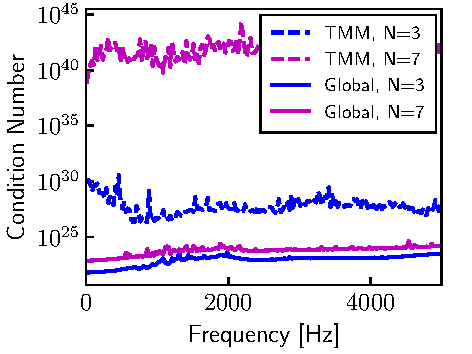
\includegraphics[width=\linewidth]{FIG/case10_condition_number.pdf}
  \caption{Condition number\label{fig:case10_CN_others}}
\end{subfigure}
\caption{Prediction of the RM and TMM for two truncation of the Bloch modes  \label{fig:case10_others}}
\end{figure}

\subsection{Automatic selection of Bloch wave numbers}
\label{sec:truncation}

In this last part, the concern of the number of Bloch modes required for an accurate solution evaluation will be dealt with. Only results from the GM are presented since it was identified as the most stable method among the different numerical strategies discussed in previous results. The multiple scattering solution will be used as reference, its Bloch modes truncation not being at stake in this discussion. In the literature, the truncating of the series uses an empirical formula that is detailed e.g. in Appendix D from Ref.~\cite{weisserAcousticBehaviorRigidly2016}. The influence on the error of the GM by varying the amount of Bloch modes accounted is shown in \cref{fig:case_7_influence_N}. The error is also presented for different orders of interpolation ranging from p = 2 to 5 and a varying mesh characteristic size. Refining the mesh quickly leads to a plateau, showing that the FEM has converged with regards to the interpolation order and mesh size. By increasing the Bloch wave truncation, the plateau decreases significantly going from N=0 to 3. The main influence of the error is thus not due to the FEM discretization but rather is mainly due to the Bloch wave truncation.

Finally, the influence of the number of accounted Bloch modes is investigated in the present section. By selecting the solution along the dashed line in \cref{fig:case_7_influence_N}, the variation of the relative error comparing a computation that accounts $N$ Bloch waves to a computation using an additional mode at $N+1$ Bloch modes is presented in \cref{fig:case7_automatic}. A plateau is reached around $N=4$, signifying that the convergence of the Bloch wave series for all shown orders of interpolation has been reached. 
This could be implemented as an automatic truncation criterion, as the evaluation of the full system accounting for additional Bloch waves is much less computationnaly intensive than evaluating the full system: the main FEM matrix does not have to be re-evaluated in this case and the LU factors of the main FEM matrix $\mat{D}_{\pi\pi}$ could be stored to evaluate the $\mat{R_b}$ and $\mat{R_t}$ from \cref{eq:rb_rt} with at a low computational cost, ensuring that the convergence is reached for the Bloch wave truncation.
\begin{figure}[hbtp]
\centering
\begin{subfigure}{.5\textwidth}
  \centering
  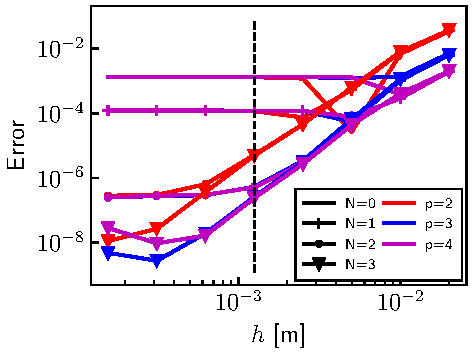
\includegraphics[width=\linewidth]{FIG/case_7_convergence_Bloch.pdf}
  \caption{Influence of the number of Bloch modes\label{fig:case_7_influence_N}}
\end{subfigure}%
\begin{subfigure}{.5\textwidth}
  \centering
  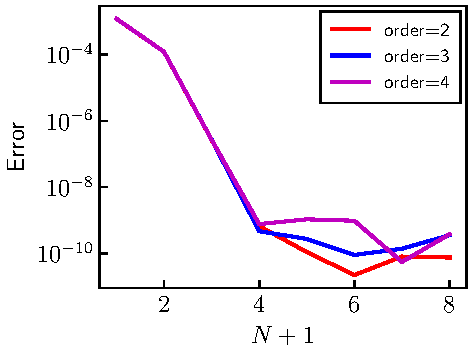
\includegraphics[width=\linewidth]{FIG/case_7_convergence_Bloch_auto.pdf}
  \caption{Differences on the errors\label{fig:case7_automatic}}
\end{subfigure}
\caption{Automatic selection of the number of Bloch modes  \label{fig:case7}}
\end{figure}


\section{Conclusion}

A stable and robust approach for the modeling of the acoustic response of grating stacks with homogeneous layers and periodic cells has been proposed in this paper. Each layer in the stack is coupled to its neighbours using the appropriate state vectors, thus allowing for the coupling of different materials  as well as non-coinciding finite elements meshes. This method has also been benchmarked against another more classical numerical approach, that is the TMM. While the TMM has been successfully coupled to high-order finite elements when modelling some of the tackled configurations spanning previous results from the literature, they exhibited limitations due to their instability for a few of the selected cases. On the other end, the GM produced satisfactory results for all presented cases, demonstrating its robustness. A criterion for the automatic evaluation of the number of required Bloch modes has been proposed as well. 

This work could be extended by proposing a full 3D extension for the problem formulation. A similar method for the stabilization of the recursive method could also be interesting, but more work is needed. Even though for this work the same extension as TMM was operated on the RM, the observed results remained unsatisfactory compared to the GM. Other prospects for this work include the declination of the methods to other physics: electromagnetics to compute the scattering properties of different types of grating stacks.

% \bibliography{comparison}
% \bibliographystyle{wileyj}
% \end{document}